\documentclass[11pt]{article}

\usepackage{lscape}

\usepackage{graphicx}
\usepackage[utf8]{inputenc}
\usepackage{amsmath}
\begin{document}
%\begin{landscape}

\begin{minipage}{0.45\textwidth}
\underline{\textbf{Grundformeln}}\\
WS: $R = \frac{U}{I} = \frac{\rho \cdot l}{A}$; $[R] = 1\frac{V}{A} =1 \Omega$ \\
Leitwert: $G = \frac{1}{R}$\\
Maschensatz: $\sum U_i = 0$\\
Knotensatz: $\sum I_i = 0$\\
Reihe WS: $R_{ges} = \sum R_i$\\
Parallel WS: $\frac{1}{R_ges} = \sum \frac{1}{R_i}$\\
\phantom{ss} Spezialfall: $R_{ges} = \frac{R_1 \cdot R_2}{R1+R2} $\\
Spannungs-Teiler: $\frac{U_1}{U_2} = \frac{R_1}{R_2}$\\
Strom-Teiler: $\frac{I_1}{I_2} = \frac{R_2}{R_1}$\\
Leistung: $P =U \cdot I = \frac{U^2}{R} = I^2 \cdot R $ \\
\phantom{ssssssssss} $[P] = 1V \cdot A =1 W$\\
\underline{\textbf{Kondensator:}}\\
Kapazität: $C = \frac{Q}{U} = \frac{\varepsilon \cdot A }{d},$\\
\phantom{ssssssssssii} $[C]=1F$\\
\phantom{sssssssssssii} $d =$ Plattenabstand\\
Ladung: $q = \int_{t_0}^t i(\tau) d\tau + q_0$\\
\phantom{sssssssis} $\stackrel{homogen}{=} I \cdot t$\\
\phantom{ssssssssssii} $[q]=1C$\\
Spannung: $U = \frac{Q}{C}$\\
\phantom{ssi} $= \frac{1}{C} \cdot (\int_{t_0}^t i(\tau) d\tau + q_0)$\\
Kond. parallel: $C_{ges} = C_1 + C_2$\\
Kond. in Reihe: $C_{ges} = C_1 || C_2$\\
Kond. in Reihe: $Q_1 = Q_2 = Q_{12}$\\
\\
$\tau = R \cdot C$\\
Zeit Auf-/Entlanden: $t = 3\tau$\\
Arbeit(=Energie): $W = \int_0^\infty P dt$\\
\phantom{sssssssss} $= \frac{U_b^2 \cdot C}{2} $
$W_{Zyklus} = W_a + W_e$\\
% TODO Wann ist aufladen mit U(1-e) und wann k1 + k2*e?

\underline{\textbf{Felder: }}\\
Stromdichte: $S=\frac{I}{A}$\\
Feldstärke: $E=\frac{S}{\kappa}$\\
Spannungsabfall: $U=E \cdot l$\\
    Potenzial: $\varphi (x)= \int_x^0 E(s)ds + \varphi(0)$\\
Stromstärke: $I = \oint H ds = H \cdot 2\pi r$\\
Magnetische Feldstärke: $H = \frac{I}{2\pi d}, [H] = 1\frac{A}{m}$\\
Kraft pro Leitungslänge: $F=Q \cdot v \cdot B, [F] = 1N$\\
Ladung pro Millimeter: $Q = \rho \cdot V, [Q] = 1C$\\
$e^-$-Geschwindigkeit: $v = \frac{S}{\rho}, [v] = 1\frac{m}{s}$\\
Flussdichte: $B=\mu \cdot H, [B] = 1 \frac{Vs}{m^2}$\\




\end{minipage}%
~~~~~~~
\begin{minipage}{0.3\textwidth}

\underline{\textbf{Maschenstromanalyse}}\\
1. Stelle Maschen auf
2. Für jede Masche Maschensatz aufstellen
3. Forme Gleichungen so um, dass alle Terme mit einem I auf einer Seite stehen, und alle ohne auf der anderen
4. $\begin{bmatrix}
	I_C\\
	I_D\\
\end{bmatrix} = \frac{1}{\sum R_iR_j} \cdot \begin{bmatrix}
	11 & 12\\ % TODO Wie ist diese Matrix aufgebaut?
	21 & 22\\
\end{bmatrix} \cdot \begin{bmatrix}
	Term~ohne~I_C\\
	Term~ohne~I_D\\
\end{bmatrix} 
 $\\
 % TODO Wie Gleichungen daraus?

\underline{\textbf{Leitungen:}}\\
$k_0 = \frac{R_w}{R_w + R_i} $\\
$r_a = \frac{R_a - R_w}{R_a + R_w} $\\
$k_a = 1 + r_a$\\
Anfang: $U_k(0,t)=k_0 \cdot U_{q1}(t)$\\
Ende: $U_k(x,t)= k_0 \cdot U_{q1}(t-\Delta t)$
Auskoppeln Gatter:\\
\phantom{ss} $U_1(t) = k_a \cdot U_1(x,t)$\\
$\Delta t = l/c$\\
%Aufladen über WS: $

\underline{\textbf{Koaxialkabel}}:\\
$R_W = \sqrt{\frac{L'}{C'}}$\\
    \phantom{sssi} $=\frac{\sqrt{\epsilon_R \cdot \mu_R}}{c_0 \cdot C'}$\\
    \phantom{sssi} $=\frac{\sqrt{\mu_R} \cdot ln(\frac{d_a}{d_i})}{2c_0 \cdot \pi \cdot \epsilon_0 \cdot \sqrt{\epsilon_R}}$\\


\end{minipage}%
~~~~~~
\begin{minipage}{0.3\textwidth}
\underline{\textbf{Operationsverstärker}}:\\
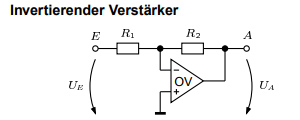
\includegraphics[scale=0.40]{IOV.png}
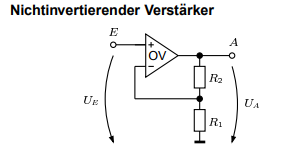
\includegraphics[scale=0.40]{NIOV.png}
$U_D = 0$
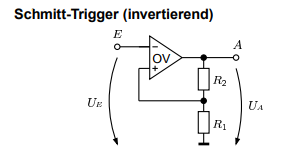
\includegraphics[scale=0.40]{ISTOV.png}
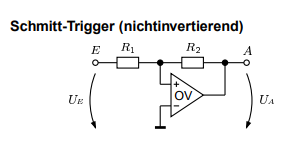
\includegraphics[scale=0.40]{NISTOV.png}
% TODO U_D = ?
\end{minipage}%

%\end{landscape}
\end{document}
